\documentclass[parskip=full]{scrartcl}
\usepackage[utf8]{inputenc} % use utf8 file encoding for TeX sources 

\usepackage[T1]{fontenc} % avoid garbled Unicode text in pdf 
\usepackage[german]{babel} % german hyphenation, quotes, etc 
\usepackage{hyperref} % detailed hyperlink/pdf configuration
\usepackage{graphicx}
\usepackage[toc]{glossaries}
\usepackage{caption}
\usepackage{pdfpages}
\hypersetup{ % ‘texdoc hyperref‘ for options 
	pdftitle={Entwurf}, %
	bookmarks=true,%
}
\usepackage{csquotes} % provides \enquote{} macro for "quotes"
\usepackage{enumitem}
\makeglossaries



\newglossaryentry{FCM}
{
	name={FCM},
	description={Firebase Cloud Messaging \href{https://firebase.google.com/docs/cloud-messaging/}{https://firebase.google.com/docs/cloud-messaging/}},
	first={Firebase Cloud Messaging(FCM)},
	long={Firebase Cloud Messaging}
}
\begin{document}
	\section{Einleitung}
		bli bla blub
	\section{Klassendiagramme}
	
		\subsection{Spiel}
		
		\begin{minipage}{\linewidth}
			\centering
			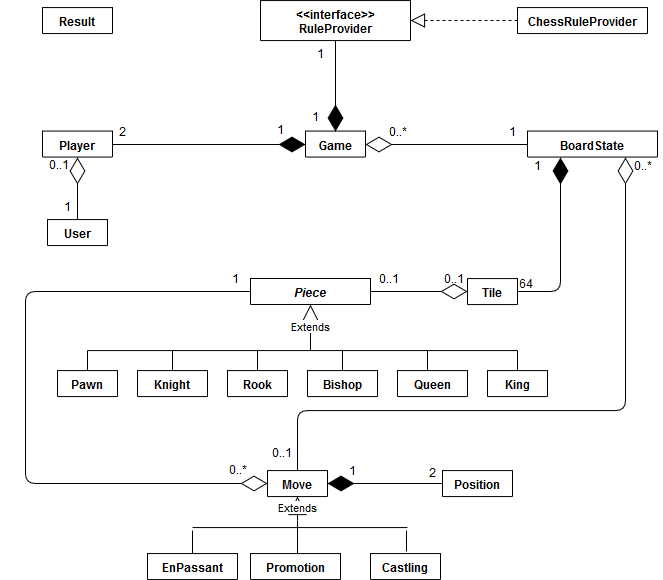
\includegraphics[width=1\linewidth]{Diagramme/TotalGame}
			\captionof{figure}{TotalGame}
			\label{fig:totalGame}
		\end{minipage}
		\begin{itemize}
			\item
				\begin{description}
				
				\end{description}
			\item
				\begin{description}
				
				\end{description}
		\end{itemize}
		\newpage
		
		\begin{minipage}{\linewidth}
			\centering
			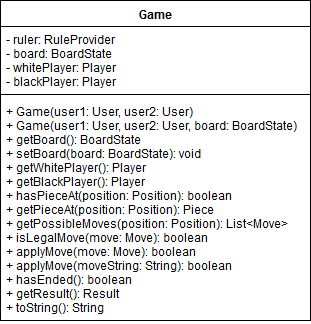
\includegraphics[width=1\linewidth]{Diagramme/Game}
			\captionof{figure}{Game}
			\label{fig:game}
		\end{minipage}
		\begin{itemize}
			\item \textbf{Game}
				\begin{description}
					 \item \textbf{\textit{ruler:}} Objekt, welches die Spielregeln zur Verfügung stellt.
					 \item \textbf{\textit{board:}} Hier wird der aktuelle Spielstatus gespeichert.
					 \item \textbf{\textit{whitePlayer:}} Der Spieler mit den weißen Figuren.
					 \item \textbf{\textit{blackPlayer:}} Der Spieler mit den schwarzen Figuren.
					 \item \textbf{\textit{Game(User, User, boolean}} Konstruktor, welcher ein Spiel mit den Standard Schachregeln erzeugt. Der boolean sagt, ob der erste User der weiße Spieler sein soll, oder ob die Farbe gewürfelt werden soll.
					 \item \textbf{\textit{getBoard():}} Gibt den Brettstatus des akutellen Spiels als Objekt zurück.
					\item \textbf{\textit{getBoard(BoardState):}} Setzt den Brettstatus neu.
					\item \textbf{\textit{getWhitePlayer():}} Gibt den weißen Spieler zurück.
					\item \textbf{\textit{getBlackPlayer():}} Gibt den schwarzen Spieler zurück.
					\item \textbf{\textit{getPossiblePositions():}} Gibt alle möglichen Positionen als Liste zurück, auf welche eine Figur, welche sich auf der übergebenen Position befindet, ziehen kann. Zum Berechnen dieser wird das ruler Objekt benutzt.
					\item \textbf{\textit{applyMove(Move):}} Führt einen übergebenen Zug auf dem Brett aus.
					\item \textbf{\textit{applyMove(String):}}Führt einen als String übergebenen Zug auf dem Brett aus. Dazu muss der String erst in ein Zugobjekt umgewandelt werden.
				\end{description}
			
		\end{itemize}		
		\newpage
		
		\begin{minipage}{\linewidth}
			\centering
			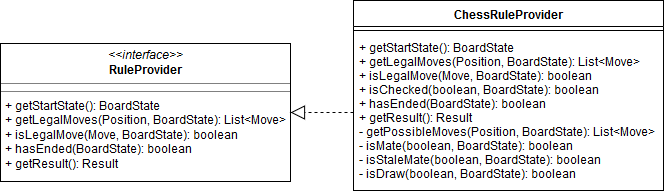
\includegraphics[width=1\linewidth]{Diagramme/RuleProvider}
			\captionof{figure}{RuleProvider}
			\label{fig:ruleProvider}
		\end{minipage}
		\begin{itemize}
			\item \textbf{RuleProvider}
				\begin{description}
				\item Interface, welches alle nötigen Regeln eines Spiels auf einem Schachbrett bereitstellt. Die zu implementierenden Methoden sind:
				\item \textbf{\textit{getStartState():}} Soll die Anfangskonfiguration eines Brettes für das jeweilige Spiel zurückgeben.
				\item \textbf{\textit{getLegalMoves(Position, BoardState):}} Soll auf einem Brett ausgehend von einer Position die Zugmöglichkeiten der sich darauf befindenden Figur berechnen, entsprechend der implementierten Regeln.
				\item \textbf{\textit{isLegalMove(Move, BoardState):}} Soll überprüfen, ob ein Zug gemäß der jeweiligen Regeln auf einem bestimmten Brett erlaubt ist.
				\item \textbf{\textit{hasEnded(BoardState):}} Soll prüfen, ob ein gegebener Zug auf dem gegebenen Brett erlaubt ist.
				\item \textbf{\textit{getResult(BoardState):}} Soll prüfen, ob ein Spiel beendet ist, wenn ja soll ein Ergebnis zurückgegeben werden, wenn nicht ein Null-Objekt.
				\end{description}
			\item \textbf{ChessRuleProvider}
				\begin{description}
				\item Konkreter Regellieferer, welcher die genauen Schachregeln zur Verfügung stellt.
				\item \textbf{\textit{getStartState():}} Gibt die Standard Anfangsstellung eines Schachspiels als BoardState zurück.
			\item\textbf{\textit{getLegalMoves(Position, BoardState):}} Gibt eine Liste an erlaubten Zügen ausgehen von einer ausgewählten Position und einem Brett zurück. Dazu werden zunächst mit \textbf{\textit{getPossibleMoves(Position, BoardState)}} alle möglichen Züge berechnet. Anschließen wird jeder Zug auf einer Kopie des Brettes simuliert, und mithilfe von \textbf{\textit{isChecked(boolean, BoardState)}} überprüft, ob der selbe Spieler danach im Schach stünde (was den Zug ungültig machen würde).
				\end{description}
				\item \textbf{\textit{isChecked(boolean, BoardState):}} Überprüft ob ein Spieler auf dem gegebenen Brett im Schach steht. Ist der übergebene boolean true, wird Weiß überprüft, bei false Schwarz. Dazu wird geschaut, ob es eine gegnerische Figur gibt, welche durch \textbf{\textit{getPosssibleMoves(Position, BoardState)}} einen Zug erhält, mit welchem der gegnerische König erreicht werden könnte.
				\item \textbf{\textit{hasEnded(BoardState():}} Prüft, ob das Schachspiel zu Ende ist. Dazu wird geprüft, ob der zu ziehende Spieler laut \textbf{\textit{isMate(boolean, BoardState)}} Matt gesetzt, laut \textbf{\textit{isStaleMate(boolean, BoardState)}} Patt gesetzt oder ob laut  \textbf{\textit{isDraw(boolean, BoardState)}} andersweitig ein Unentschieden erreicht wurde.
				\item \textbf{\textit{getResult()}} Ruft \textbf{\textit{hasEnded(BoardState)}} auf, gibt aber bei beendetem Spiel das jeweilige Ergebnis als Result mit Begründung zurück. Ist das Spiel nicht beendet wird null zurückgegeben.
				\item \textbf{\textit{getPossibleMoves(Position, BoardState):}} Gibt alle möglichen Züge einer Figur auf dem Brett zurück, ohne dabei zu berücksichtigen, ob der ziehende Spieler nach diesem Zug im Schach stehen würde.
				\item \textbf{\textit{isMate(boolean, BoardState):}} Prüft, ob der übergebene Spieler Matt gesetzt wurde. Das ist der Fall, wenn der Spieler laut \textbf{\textit{isChecked(boolean, BoardState)}} im Schach steht, und es für keine Figur einen nach \textbf{\textit{getLegalMoves(Position, BoardState)}}erlaubten Zug gibt.
				\item \textbf{\textit{isStaleMate(boolean, BoardState):}} Prüft, ob der übergebene Spieler Patt gesetzt wurde. Das ist der Fall, wenn der Spieler laut \textbf{\textit{isChecked(boolean, BoardState)}} nicht im Schach steht, und es für keine Figur einen nach \textbf{\textit{getLegalMoves(Position, BoardState)}}erlaubten Zug gibt.
				\item \textbf{\textit{isDraw(boolean, BoardState):}} Prüft, ob ein anderweitiges Unentschieden erreicht wurde. Dies ist der Fall, wenn zu wenig Figuren auf dem Brett vorhanden sind, um Matt zu setzen, oder wenn 50 Züge lang keine Figur geschlagen und kein Bauer gezogen wurde.
		\end{itemize}
		\newpage

\begin{minipage}{\linewidth}
			\centering
			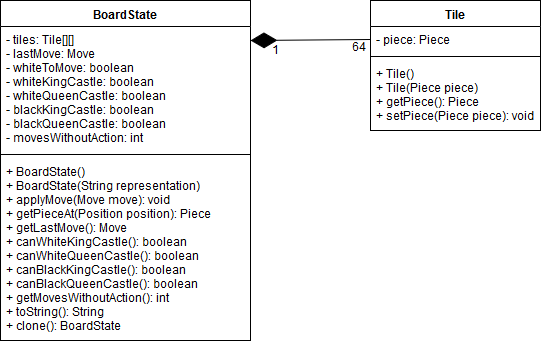
\includegraphics[width=1\linewidth]{Diagramme/BoardState}
			\captionof{figure}{BoardState}
			\label{fig:boardState}
		\end{minipage}
		\begin{itemize}
			\item \textbf{\textit{BoardState}}
				\begin{description}
				\item Der gesamte Status eines Schachspiels er notwendig ist, um alle Regeln überprüfen zu können.
				\item \textbf{\textit{tiles:}} Ein Array von Tiles, welches den Aufbau des Spielbretts darstellt
				 \item \textbf{\textit{lastMove:}} Der letzte gespielte Zug.
				 \item \textbf{\textit{whiteToMove:}} Speichert, ob Weiß am Zug ist.
				 \item \textbf{\textit{whiteKingCastle:}} Speichert ab, ob Weiß noch auf der Königsseite rochieren kann.
				 \item \textbf{\textit{whiteQueenCastle:}} Speichert ab, ob Weiß noch auf der Damenseite rochieren kann.
				 \item \textbf{\textit{blackKingCastle:}} Speichert ab, ob Schwarz noch auf der Königsseite rochieren kann.
				 \item \textbf{\textit{blackQueenCastle:}} Speichert ab, ob Schwarz noch auf der Damenseite rochieren kann.
				\item \textbf{\textit{movesWithoutAction:}} Speichert die Anzahl der Züge in Folge, in welcher kein Bauer gezogen und keine Figur geschlagen wurde.
				\item \textbf{\textit{BaordState():}} Erzeugt ein leeres Schachbrett und setzt alle Variablen auf ihre Standardwerte.
				\item \textbf{\textit{BoardState(String):}} Erzeugt ein Brett, ausgehen von einem String. In diesem müssen alle notwenidigen Informationen in einem bestimmten Format gespeichert sein.
				\item \textbf{\textit{applyMove(Move):}} Führt einen Zug auf dem Brett aus, indem es die Figur(en) wie im Move-Objekt vorgegeben bewegt.
				\item \textbf{\textit{getPieceAt(Position):}} Gibt die Figur an einer Position zurück.
				\item \textbf{\textit{setPieceAt(Position, Piece):}} Setzt eine Figur an eine bestimmte Position.
				\item \textbf{\textit{getLastMove():}} Gibt \textbf{\textit{lastMove}} zurück.
				 \item \textbf{\textit{canWhiteKingCastle:}} Gibt zurück, ob Weiß noch auf der Königsseite rochieren kann.
				 \item \textbf{\textit{canWhiteQueenCastle:}} Gibt zurück, ob Weiß noch auf der Damenseite rochieren kann.
				 \item \textbf{\textit{canBlackKingCastle:}} Gibt zurück, ob Schwarz noch auf der Königsseite rochieren kann.
				 \item \textbf{\textit{canBlackQueenCastle:}} Gibt zurück, ob Schwarz noch auf der Damenseite rochieren kann.
				 \item \textbf{\textit{getMovesWithoutAction):}} Gibt \textbf{\textit{movesWithoutAction}} zurück.
				 \item \textbf{\textit{toString()}} Gibt den gesamten Brettzustand als String codiert zurück. Aus diesem String muss mithilfe des Konstruktors ein identisches Brett erzeugt werden können.			
				
				\end{description}
			\item \textbf{\textit{Tile}}
				\begin{description}
				\item Stellt eine Feld eines Schachbretts dar.
				\item \textbf{\textit{piece}} Die Figur, welche sich auf dem Feld befindet. Befindet sich keine Figur auf dem Feld, steht hier null.
				\item \textbf{\textit{Tile():}} Konstruktor, welcher ein leeres Feld erzeugt.
				\item \textbf{\textit{Tile(Piece):}} Konstruktor, welcher ein Feld mit der übergebenen Figur darauf erzeugt.
				\item \textbf{\textit{getPiece():}} Gibt \textbf{\textit{piece}} zurück.
				
				\end{description}
		\end{itemize}
		\newpage		
		
\begin{minipage}{\linewidth}
			\centering
			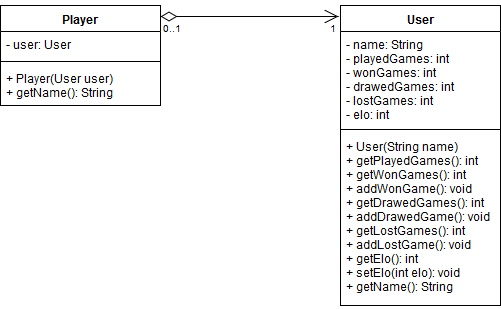
\includegraphics[width=1\linewidth]{Diagramme/Player}
			\captionof{figure}{Player}
			\label{fig:player}
		\end{minipage}
		\begin{itemize}
			\item
				\begin{description}
				
				\end{description}
			\item
				\begin{description}
				
				\end{description}
		\end{itemize}
		\newpage		
		
		\begin{minipage}{\linewidth}
			\centering
			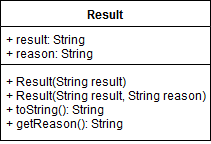
\includegraphics[width=1\linewidth]{Diagramme/Result}
			\captionof{figure}{Result}
			\label{fig:result}
		\end{minipage}
		\begin{itemize}
			\item
				\begin{description}
				
				\end{description}
			\item
				\begin{description}
				
				\end{description}
		\end{itemize}
		\newpage
		
		\begin{minipage}{\linewidth}
			\centering
			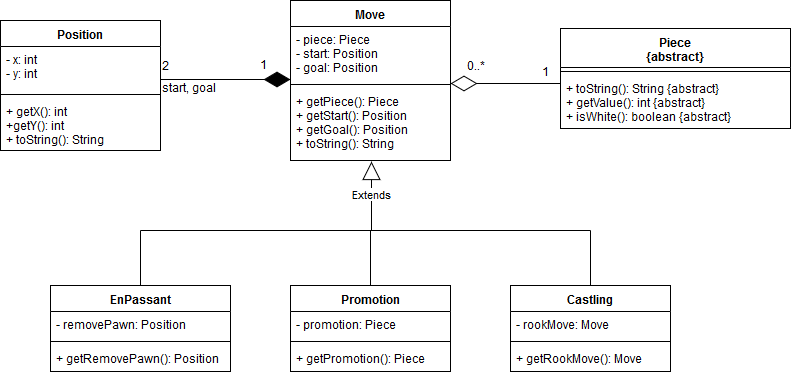
\includegraphics[width=1\linewidth]{Diagramme/Move}
			\captionof{figure}{Move}
			\label{fig:move}
		\end{minipage}
		\begin{itemize}
			\item
				\begin{description}
				
				\end{description}
			\item
				\begin{description}
				
				\end{description}
		\end{itemize}
		\newpage
		
		\begin{minipage}{\linewidth}
		\centering
		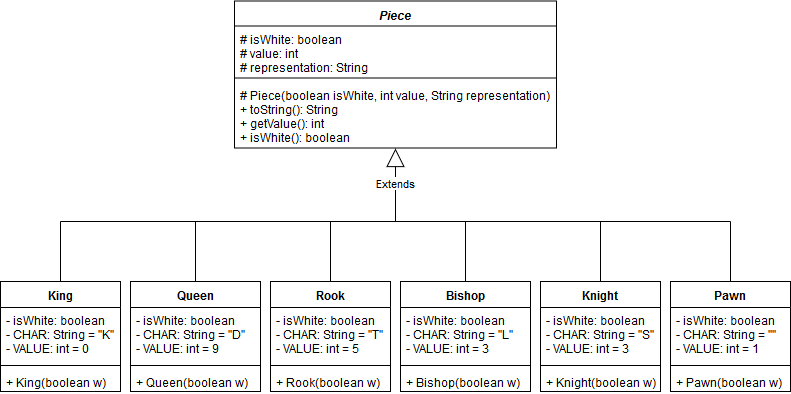
\includegraphics[width=1\linewidth]{Diagramme/Pieces}
		\captionof{figure}{Pieces}
		\label{fig:pieces}
		\end{minipage}
		\begin{itemize}
			\item
				\begin{description}
				
				\end{description}
			\item
				\begin{description}
				
				\end{description}
		\end{itemize}		
		\newpage		
		
		\subsection{GUI}
		
		\newpage
		\subsection{Server}
		\begin{minipage}{\linewidth}
			\centering
			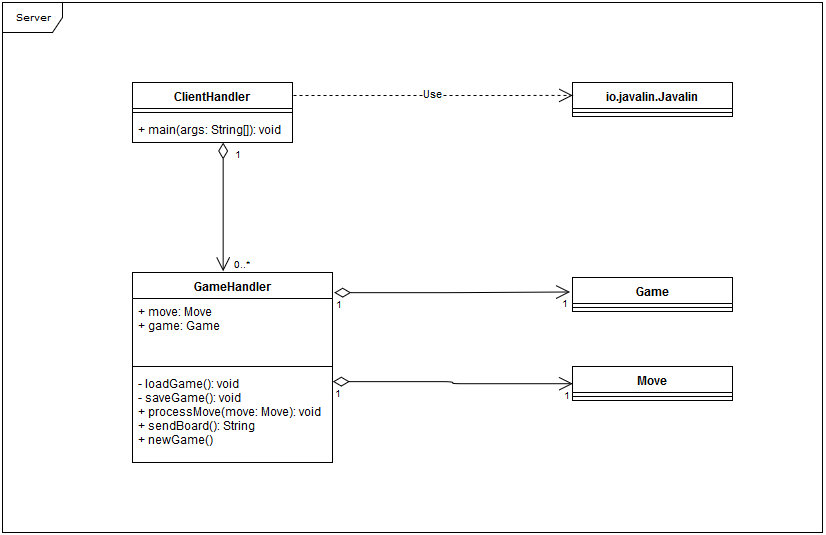
\includegraphics[width=1\linewidth]{Diagramme/Server}
			\captionof{figure}{Server}
			\label{fig:server}
		\end{minipage}
		\begin{itemize}
			\item \textbf{ClientHandler}
			Verwaltet eingehende Anfragen an den Server.
			\begin{description}
				\item \textbf{\textit{main(String[] args):}}
				Die main Methode des Servers. Hier wird der Javalin Server gestartet und für jede Anfrage ein neues GameHandler Objekt erzeugt. Diesem werden die gesendeten Anfragen übermittelt. 
			\end{description} 
	
	
			\item \textbf{GameHandler}
			\begin{description}
				\item \textbf{\textit{Move move:}}
				Der Zug, den der GameHandler übermittelt bekommen hat.
				\item \textbf{\textit{Game game:}}
				Das Spiel, das aus der Datenbank geladen wurde.
				\item \textbf{\textit{loadGame():}}
				Lädt das aktuelle Spiel des Spielers aus der Datenbank und erzeugt daraus ein Game Objekt.
				\item \textbf{\textit{saveGame():}}
				Speichert das Game Objekt wieder als String in der Datenbank ab.
				\item \textbf{\textit{processMove():}}
				Führt zuerst loadGame() aus, überprüft den gegebenen Zug auf Gültigkeit, wendet diesen an, sendet ihn an den anderen Spieler und führt anschließend saveGame() aus.
				\item \textbf{\textit{sendBoard():}}
				Sendet das Brett des Spiels per \gls{FCM}.
				\item \textbf{\textit{newGame():}}
				Legt einen neuen Eintrag in der Datenbank an und füllt ihn mit beiden Benutzernamen und der Startposition.
			
			\end{description} 
		\end{itemize}
	\section{Sequenzdiagramm}
\printglossaries
\end{document}